%\documentclass[a4paper, 10pt, conference]{../../templates/IEEEconf/IEEEconf}
\documentclass[10pt, onecolumn, conference]{../../../templates/IEEEtran/IEEEtran}
%\documentclass[10pt, journal]{../../templates/IEEEtran/IEEEtran}

\usepackage{graphicx}
\usepackage{caption} 
\usepackage{subcaption}
\usepackage{hyperref}
\usepackage{listings}
\usepackage{hhline}
\usepackage{float}
\usepackage{amssymb}
\usepackage[autostyle=true]{csquotes}
\usepackage{amsmath}
\usepackage{marvosym}
\usepackage{minted}

%\font\subtitlefont=cmr12 at 18pt
%
\title{Towards pure functional agent-based simulation}

% IEEEtran journal authors
%\author{Jonathan Thaler, ̃Peer-Olaf Siebers \\ School of Computer Science \\ University of Nottingham%
%\thanks{jonathan.thaler@nottingham.ac.uk}%
%\thanks{peer-olaf.siebers@nottingham.ac.uk}
%}

%IEEEtran conference authors
\author{
	\IEEEauthorblockN{Jonathan Thaler}
	\IEEEauthorblockA{School of Computer Science\\
		University of Nottingham\\
		jonathan.thaler@nottingham.ac.uk}
		
	\and
		
	\IEEEauthorblockN{Peer-Olaf Siebers}
	\IEEEauthorblockA{School of Computer Science\\
		University of Nottingham\\
		peer-olaf.siebers@nottingham.ac.uk}
}

%\IEEEpubid{0000--0000/00\$00.00 ̃\copyright ̃2015 IEEE}

% IEEEconf authors
%\author{
%	Jonathan Thaler \\
%	\email{jonathan.thaler@nottingham.ac.uk} \\
%	\begin{affiliation}
%		School of Computer Science, University of Nottingham
%	\end{affiliation} \\
%	\and 
%	Peer-Olaf Siebers \\
%	\email{peer-olaf.siebers@nottingham.ac.uk} \\
%	\begin{affiliation}
%		School of Computer Science, University of Nottingham
%	\end{affiliation} 
%	\and 
%	Thorsten Altenkirch \\
%	\email{thorsten.altenkirch@nottingham.ac.uk} \\
%	\begin{affiliation}
%		School of Computer Science, University of Nottingham
%	\end{affiliation} 
%}

\begin{document}
\maketitle 

\begin{abstract}
So far, the pure functional paradigm hasn't got much attention in Agent-Based Simulation (ABS) where the dominant programming paradigm is object-orientation, with Java, Python and C++ being its most prominent representatives. We claim that pure functional programming using Haskell is very well suited to implement complex, real-world agent-based models and brings with it a number of benefits. To show that we implemented the seminal Sugarscape model in Haskell in our library \textit{FrABS} which allows to do ABS the first time in the pure functional programming language Haskell. To achieve this we leverage the basic concepts of ABS with functional reactive programming using Yampa. The result is a surprisingly fresh approach to ABS as it allows to incorporate discrete time-semantics similar to Discrete Event Simulation and continuous time-flows as in System Dynamics. In this paper we will show the novel approach of functional reactive ABS through the example of the SIR model, discuss implications, benefits and best practices.
\end{abstract}

\begin{IEEEkeywords}
Haskell, Functional Programming, Verification
\end{IEEEkeywords}

\section{Introduction}
There exists a large number of simulation packages which allow the convenient creation of System Dynamics simulations by straight-forward visual diagram creation. One simply creates stocks and flows, connects them, specifies the flow-rates and initial parameters and then runs the model. An example for such a visual diagram creation in the simulation package AnyLogic can be seen in Figure \ref{fig:sir_stockflow_diagram}.

\begin{figure}
	\centering
	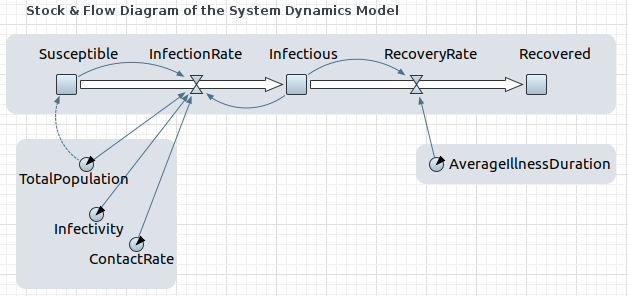
\includegraphics[width=.5\textwidth, angle=0]{./fig/SIR_SD_STOCKFLOW_DIAGRAMM.png}
	\caption{Visual System Dynamics Diagram of the SIR model in AnyLogic Personal Learning Edition 8.3.1.}
	\label{fig:sir_stockflow_diagram}
\end{figure}

Still, implementing System Dynamics directly in code is not as straight forward and involves numerical integration which can be quite tricky to get right. Thus, the aim of this paper is to look into how System Dynamics models can be implemented in code correctly without the use of a simulation package. We use the well known SIR model \cite{kermack_contribution_1927} from epidemiology to demonstrate our approach.

Our language of choice is Haskell because it emphasises a declarative programming style in which one describes \textit{what} instead of \textit{how} to compute. Further it allows to rule out interference with non-deterministic influences or side-effects already at compile-time. This is of fundamental importance for System Dynamics because it behaves completely deterministic and involves no stochastics or non-determinism whatsoever. Also, we make use of Functional Reactive Programming which allows to express continuous-time systems in a functional way. 

We show that by this approach we can arrive at correct-by-construction implementations of System Dynamic models. This means that the correctness of the code is obvious because we have closed the gap between the model specification and its implementation. Thus, the contribution of the paper is the demonstration of how to implement correct-by-construction System Dynamics simulations using Haskell and Functional Reactive Programming.

\section{Agent-Based Simulation Defined}
Agent-Based Simulation (ABS) is a methodology to model and simulate a system where the global behaviour may be unknown but the behaviour and interactions of the parts making up the system is of knowledge. Those parts, called agents, are modelled and simulated out of which then the aggregate global behaviour of the whole system emerges. Epstein \cite{epstein_generative_2012} identifies ABS to be especially applicable for analysing \textit{"spatially distributed systems of heterogeneous autonomous actors with bounded information and computing capacity"}. Thus in the line of the simulation methods \textit{Statistic} $^\dag$, \textit{Markov} $^\ddag$, \textit{System Dynamics} $^\S$, \textit{Discrete Event} $^\mp$, ABS is the most recent development and the most powerful one as it subsumes it's predecessors features and goes beyond:

\begin{itemize}
	\item Linearity \& Non-Linearity $^{\dag \ddag \S \mp}$ - the dynamics of the simulation can exhibit both linear and non-linear behaviour. 
	\item Time $^{\dag \ddag \S \mp}$ - agents act over time, time is also the source of pro-activity.
	\item States $^{\ddag \S \mp}$ - agents encapsulate some state which can be accessed and changed during the simulation.
	\item Feedback-Loops $^{\S \mp}$ - because agents act continuously and their actions influence each other and themselves, feedback-loops are the norm in ABS. 
	\item Heterogeneity $^{\mp}$ - although agents can have same properties like height, sex,... the actual values can vary arbitrarily between agents.
	\item Interactions - agents can be modelled after interactions with an environment or other agents, making this a unique feature of ABS, not possible in the other simulation models.
	\item Spatiality \& Networks - agents can be situated within e.g. a spatial (discrete 2d, continuous 3d,...) or network environment, making this also a unique feature of ABS, not possible in the other simulation models.
\end{itemize}

\subsection{Deriving central concepts}
Before we can approach a functional view on ABS, we need to identify the central concepts of ABS on a more technical level. Unfortunately there does not exist a commonly agreed technical definition of ABS but we can draw inspiration from the closely related field of Multi-Agent Systems (MAS). It is important to understand that MAS and ABS are two different fields where in MAS the focus is much more on technical details implementing a system of interacting intelligent agents within a highly complex environment with the focus primarily on solving AI problems.

\subsubsection{Agents}
The central aspect of ABS is the concept of an agent. In MAS \cite{wooldridge_introduction_2009}, \cite{weiss_multiagent_2013} agents can be informally defined as:

\begin{itemize}
	\item They are uniquely addressable entities with some internal state over which they have full, exclusive control.
	\item They are situated in an environment which they can observe and act upon.
	\item They can interact with other agents which are situated in the same environment.
	\item They are pro-active which means they can initiate actions on their own e.g. change their internal state, interact with other agents, create new agents, terminate themselves, interact with the environment,...
\end{itemize}

\subsubsection{Environment}
The other important concept is the one of an environment. In MAS \cite{wooldridge_introduction_2009}, \cite{weiss_multiagent_2013} one distinguishes between different types of environments (based on \cite{russell_artificial_2010}):

\begin{itemize}
	\item Accessible vs. inaccessible - in an accessible environment an agent can obtain complete and accurate information from the environment. In ABS environments are generally implemented as being accessible.
	\item Deterministic vs. non-deterministic - in a deterministic environment the actions of an agent have no uncertainty and are guaranteed to have a single effect. In ABS environments are generally implemented as being deterministic.
	%\item Episodic vs. non-episodic - in an episodic environment agents act only on the current state and do not project into the future. In ABS environments are generally episodic.
	\item Static vs. dynamic - a static environment only changes due to the agents actions whereas a dynamic one has other processes which operate on it. In ABS both static and dynamic environments are common.
	\item Discrete vs. continuous - a discrete environment has only a fixed, finite number of states and actions whereas a continuous is potentially unlimited. In ABS both discrete and continuous environments are common.
\end{itemize}

Note that in MAS the focus is much more on the environment rather than on the agents where the environment is almost always a highly complex one and the agents may intelligently act on it. In ABS the focus is rather on the agents and their interactions where the environment plays a role but is not of central interest as it is almost always deterministic.

\subsection{Deriving a formal view}
In order to explore how we can implement an ABS in a pure functional way we need a sufficiently formal view on it. This will help us expressing the concepts in Haskell as formal, mathematical specifications translate easily into functional programming. There exists formalisations of MAS \cite{wooldridge_introduction_2009} but unfortunately they are not very helpful in our context as its formalization is tailored much more towards optimizing, intelligent and reasoning behaviour of agents within a highly complex and uncertain environment. What we need for ABS is a more agent-oriented approach: 

\begin{enumerate}
	\item An ABS is a simulation over time in which time is advanced either in discrete or continuous time-steps where discrete means advancing by a natural number time-delta and continuous by a real-valued time-delta. So we have a potentially infinite stream of time-steps starting at t=0 advancing by some fixed time-delta.
	\item At each time-step all agents are allowed to act which is the source of their proactivity because it allows them to initiate actions on their own. Of course such actions are always time-dependent - be it explicitly like executing actions \textit{after} a specific time, or be it implicit like executing actions every time-delta - but this is the only way of implementing proactivity in a computer system.
	\item In each step an agent should be able to read/write the environment. TODO: orderings? when are changes visible?
	\item In each step an agent should be able to interact with other agents through communication. 
	\item In each step an agent should be able to update its internal state.
	\item Depending on its type, the environment must also be allowed to act in each time-step.
	\item In general we can thus see an agent to exhibit both time-dependent and reactive behaviour: it can act continuously or discretely, depending on how the time is advanced and exhibit reactive behaviour which means it can react to changing environment or agents.
	\item The interactions between agents their update-state and environment forms a feedback as the state of time ti forms the input state on which to act at time-step ti+1
\end{enumerate}

\section{A functional approach}
Due to the fundamentally different approaches of pure Functional Programming (pure FP) an ABS needs to be implemented fundamentally different as well compared to traditional object-oriented approaches (OO). We face the following challenges:

\begin{enumerate}
	\item How can we represent an Agent? \\
	In OO the obvious approach is to map an agent directly onto an object which encapsulates data and provides methods which implement the agents actions. Obviously we don't have objects in pure FP thus we need to find a different approach to represent the agents actions and to encapsulate its state.
	
	\item How can we represent state in an Agent? \\
	In the classic OO approach one represents the state of an Agent explicitly in mutable member variables of the object which implements the Agent. As already mentioned we don't have objects in pure FP and state is immutable which leaves us with the very tricky question how to represent state of an Agent which can be actually updated.
	
	\item How can we implement proactivity of an Agent? \\
	In the classic OO approach one would either expose the current time-delta in a mutable variable and implement time-dependent functions or ignore it at all and assume agents act on every step. At first this seems to be not a big deal in pure FP but when considering that it is yet unclear how to represent Agents and their state, which is directly related to time-dependent and reactive behaviour it raises the question how we can implement time-varying and reactive behaviour in a purely functional way.
	
	\item How can we implement the agent-agent interaction? \\
	In the classic OO approach Agents can directly invoke other Agents methods which makes direct Agent interaction \textit{very} easy. Again this is obviously not possible in pure FP as we don't have objects with methods and mutable state inside.
		
	\item How can we represent an environment and its various types? \\
	In the classic OO approach an environment is almost always a mutable object which can be easily made dynamic by implementing a method which changes its state and then calling it every step as well. In pure FP we struggle with this for the same reasons we face when deciding how to represent an Agent, its state and proactivity.
	
	\item How can we implement the agent-environment interaction? \\
	In the classic OO approach agents simply have access to the environment either through global mechanisms (e.g. Singleton or simply global variable) or passed as parameter to a method and call methods which change the environment. Again we don't have this in pure FP as we don't have objects and globally mutable state.
	
	\item How can we step the simulation? \\
	In the classic OO approach agents are run one after another (with being optionally shuffled before to uniformly distribute the ordering) which ensures mutual exclusive access in the agent-agent and agent-environment interactions. Obviously in pure FP we cannot iteratively mutate a global state.
\end{enumerate}

\subsection{Agent representation, state and proactivity}
Whereas in imperative programming (the OO which we refer to in this paper is built on the imperative paradigm) the fundamental building block is the destructive assignment, in FP the building blocks are obviously functions which can be evaluated.
Thus we have no other choice than to represent our Agents using a function which implements their behaviour. This function must be time-aware somehow and allow us to react to time-changes and inputs. Fortunately there exists already an approach to time-aware, reactive programming which is termed Functional Reactive Programming (FRP). This paradigm has evolved over the year and current modern FRP is built around the concept of a signal-function which transforms an input-signal into an output-signal. An input-signal can be seen as a time-varying value. Signal-functions are implemented as continuations which allows to capture local state using closures. Modern FRP also provides feedback functions which provides convenient methods to capture and update local state from the previous time-step with an initial state provided at time = 0.


- time is represented using the FRP concept: Signal-Functions which are sampled at (fixed) time-deltas, the dt is never visible directly but only reflected in the code and read-only.
- no method calls => continuous data-flow instead
	
Viewing agent-agent interaction as simple method calls implies the following:
- it takes no time
- it has a synchronous and transactional character
- an agent gives up control over its data / actions or at least there is always the danger that it exposes too much of its interface and implementation details. 
- agents equals objects, which is definitely NOT true. Agents 

data-flow
synchronous agent transactions

- still need transactions between two agents e.g. trading occurs over multiple steps (makeoffer, accept/refuse, finalize/abort) 
		-> exactly define what TX means in ABS
			-> exclusive between 2 agents
			-> state-changes which occur over multiple steps and are only visible to the other agents after the TX has commited
			-> no read/write access to this state is allowed to other agents while the TX is active
			-> a TX executes in a single time-step and can have an arbitrary number of tx-steps
		-> it is easily possible using method-calls in OOP but in our pure functional approach it is not possible
		-> parallel execution is being a problem here as TX between agents are very easy with sequential
		-> an agent must be able to transact with as many other agents as it wants to in the same time-step
		-> no time passes between transactions
		=> what we need is a 'all agents transact at the same time'
			-> basically we can implement it by running the SFs of the agents involved in the TX repeatedly with dt=0 until there are no more active TXs
			-> continuations (SFs) are perfectly suited for this as we can 'rollback' easily by using the SF before the TX has started
		
\subsection{Environment representation and interaction}

no global shared mutable environment, having different options:
- non-active read-only (SIR): no agent, as additional argument to each agent
- pro-active read-only (?): environment as agent, broadcast environment updates as data-flow
- non-active read/write (?): no agent, StateT in agents monad stack
- pro-active read/write (Sugarscape): environment as agent, StateT in agents monad stack

care must be taken in case of agent-transactions: when aborting/refusing all changes to the environment must be rolled back => instead of StateT use a transactional monad which allows us to revert changes to a save point at the start of the TX. if we drag the environment through all agents then we could easily revert changes but that then requires to hard-code the environment concept deep into the simulation scheduling/stepping which brings lots of inconveniences, also it would need us to fold the resulting multiple environments back into a single. If we had an environment-centric view then probably this is what we want but in ABS the focus is on the agents

question is if the TX sf runs in the same monad aw the agent or not. i opt for identity monad which prevents modification of the Environment in a transaction

also need to motivate the dt=0 in all TX processing: conceptually it all happens instantaneously (although arbitration is sequential) but agents must act time-sensitive

for environment we need transactional and shared state behaviour where we can have mutual exclusive access to shared data but also roll back changes we made. it should run deterministic when running agents not truly parallel. solution: run environment in a transactional state monad (TX monad). although the agents are executed in parallel in the end it (map) runs sequentially. this passes a mutable state through all agents which can act on it an roll back actions e.g. in case of a failed agent TX. if we dont need transactional behaviour then just use StateT monad. this ensures determinism. pro active environment is also easily possible by writing to the state. this approach behaves like sequential transactional although the agents run in parallel but how is this possible when using mapMSF ?

\subsection{Stepping the simulation}

- parallel update only, sequential is deliberately abandoned due to:
		-> reality does not behave this way
		-> if we need transactional behaviour, can use STM which is more explicit
		-> it is translates directly to a map which is very easy to reason about (sequential is basically a fold which is much more difficult to reason about)
		-> is more natural in functional programming
		-> it exists for 'transactional' reasons where we need mutual exclusive access to environment / other agents
			-> we provide a more explicit mechanism for this: Agent Transactions
			

\section{Examples}
TODO: the main punch is that our approach combines the best of the three simulation methodologies:
	- SD part: 	it can represent continuous time (as well as discrete) with continuous data-flows from agents which act at the same time (parallel update), can express the formulas directly in code, there exists also a small EDSL for expressing SD in our approach, can guarantee reproducibility and no drawing of random-numbers in our approach
		-> drawback over real SD: none known so far 
	- DES part: it can represent discrete time with events occurring at discrete points in time which cause an instant change in the system
		-> drawback over real DES: time does not advance discretely to the next event which results of course not in the performance of a real DES system
	- ABS part:	the entities of the system (=agents) can be heterogenous and pro-active in time and can have arbitrary neighbourhood (2d/3d discrete/continuous, network,...)
		-> drawback over classic ABS: none known so far 

TODO: give examples of all 3 approaches: SD \& ABS: SIR model, DES: simulation of a queuing system

In the course of the research for this paper we implemented the library \textit{Chimera} \footnote{The library is freely available on GitHub: \url{https://github.com/thalerjonathan/chimera}. It is planned that it will be put on Hackage in the future.} in Haskell which implements all the concepts introduced in this paper and allows to do ABS in a pure functional way in Haskell. As use-cases to drive the research and test our concepts we implemented a number of more or less well known examples from ABS, see Appendix \ref{app:examples} for a list of all the examples and the concepts used.

\subsection{Example I: System Dynamics SIR Model}

\subsection{Example II: Agent-Based SIR Model}

\subsection{Example III: Discrete Event Simulation}
generally a DES system is fixed in advance: the various DES objects are connected and communicate with each other through their ports. can we do this in our approach as well?

\section{Discussion}
Although there are similarities to the work of \cite{botta_time_2010} (the use of messages and the problem of when to advance time in models with arbitrary number synchronised agent-interactions), we approach our agents differently. First in our approach an agent is only a single MSF and thus can not be directly queried for its internal state / its id or outgoing messages, instead of taking a list of messages, our agents take a single event/message and can produce an arbitrary number of outgoing messages together with an observable state - note that this would allow to query the agent for its id and its state as well by simply sending a corresponding message to the agents MSF and requiring the agent to implement message handling for it. Also the state of our agents is \textit{completely} localised and there is no means of accessing the state from outside the agent, they are thus "fully encapsulated agents" \cite{botta_time_2010}. Note that the authors of \cite{botta_time_2010} define their agents with a polymorphic agent-state type \textit{s}, which implies that without knowledge of the specific type of \textit{s} there would be no way of accessing the state, rendering it in fact also fully encapsulated. The problem of advancing time in our approach is solved not exactly the same but conceptually it is the same: after sending a tick message to each agent (in random order), we process all agents until they are idle: there are no more enqueued messages / events in the queue.

our eventdriven approach makes heavy use of 2 state monads, thus one might ask what the benefits are, after all we seem to fall back into stateful, imperative style programming. we agree that our approach is just one way of implementing abs in fp but we think we have come a long way thus making our approach quite valuable even if there might be other approaches like shallow EDSLs. on the other hand even our stateful programming is highly restricted to only those 2 local datatypes which makes it much more manageable than unrestricted data mutation

quote carmack (\url{http://www.gamasutra.com/view/news/169296/Indepth_Functional_programming_in_C.php}): the main difficulty as a developer in software programming is to keep track of the states a program can be in and reason about them and their Validity

TODO: report LoC and compare it with other implementations we found on the internet

\chapter{Conclusions}
\label{chap:concl}

\section{Being Realistic}
It is of most importance to stress that we don't condemn the current state-of-the-art approach of object-oriented specification and implementation to ABS. The strength of object-oriented programming is surely that it can be seen as \textit{programming as modelling} and thus will be always an attractive approach to ABS. Also we are realists and know that there are more points to consider when selecting a set of methods for developing software for an ABS than robustness, verification and validation. Almost always the popularity of an existing language and which languages the implementer knows is the driving force behind which methods and languages to choose. This means that ABS will continue to be implemented in object-oriented programming languages and many perfectly well functioning models will be created by it in the future. Although they all suffer from the same issues mentioned in the introduction this doesn't matter as they are not of central importance to most of them.
Nonetheless we think our work is still essential and necessary as it may start a slow paradigm-shift and opens up the minds of the ABS community to a more functional and formal way of approaching and implementing agent-based models and simulations and recognizing the benefits one gets automatically from it by doing so.

\section{What we are not doing}
Because of this highly interdisciplinary topic we explicitly mention what we do not want to undertake in this PhD.
First we don't want to develop another language for formal agent-specification which needs to be compiled or used in some fancy tool - we want to put it directly into Haskell, building on the existing facilities.
Second, we are not developing a new economic theory about decentralized bilateral bartering, we take the existing theory and existing agent-based models and apply our methods to them.
Third, we don't want to use fancy statistics and number juggling for comparing validating and verifying models: we want structural comparison (category-theory).
Fourth, we do NOT want to do a direct comparison of object-orientation vs. functional in ABS, as we would get lost in an infinite amount of low-level technical details. We look at the benefits / drawbacks more on a conceptual level, applied to ABS.

\section*{Acknowledgments}
The authors would like to thank I. Perez, H. Nilsson, J. Greensmith, T. Schwarz and H. Vollbrecht for constructive comments and valuable discussions.

\bibliographystyle{../../../templates/IEEEtran/bibtex/IEEEtran}
\bibliography{../../../../references/phdReferences.bib}

\appendices

\newpage
\section{Examples}
TODO: the main punch is that our approach combines the best of the three simulation methodologies:
	- SD part: 	it can represent continuous time (as well as discrete) with continuous data-flows from agents which act at the same time (parallel update), can express the formulas directly in code, there exists also a small EDSL for expressing SD in our approach, can guarantee reproducibility and no drawing of random-numbers in our approach
		-> drawback over real SD: none known so far 
	- DES part: it can represent discrete time with events occurring at discrete points in time which cause an instant change in the system
		-> drawback over real DES: time does not advance discretely to the next event which results of course not in the performance of a real DES system
	- ABS part:	the entities of the system (=agents) can be heterogenous and pro-active in time and can have arbitrary neighbourhood (2d/3d discrete/continuous, network,...)
		-> drawback over classic ABS: none known so far 

TODO: give examples of all 3 approaches: SD \& ABS: SIR model, DES: simulation of a queuing system

In the course of the research for this paper we implemented the library \textit{Chimera} \footnote{The library is freely available on GitHub: \url{https://github.com/thalerjonathan/chimera}. It is planned that it will be put on Hackage in the future.} in Haskell which implements all the concepts introduced in this paper and allows to do ABS in a pure functional way in Haskell. As use-cases to drive the research and test our concepts we implemented a number of more or less well known examples from ABS, see Appendix \ref{app:examples} for a list of all the examples and the concepts used.

\subsection{Example I: System Dynamics SIR Model}

\subsection{Example II: Agent-Based SIR Model}

\subsection{Example III: Discrete Event Simulation}
generally a DES system is fixed in advance: the various DES objects are connected and communicate with each other through their ports. can we do this in our approach as well?

\newpage
\section{Functional-Reactive code of the System-Dynamics SIR model}
\label{app:sd_code}

\begin{minted}[fontsize=\footnotesize, linenos]{haskell}
totalPopulation :: Double
totalPopulation = 1000

infectivity :: Double
infectivity = 0.05

contactRate :: Double
contactRate = 5

avgIllnessDuration :: Double
avgIllnessDuration = 15

-- Hard-coded ids for stocks & flows interaction
susceptibleStockId :: StockId
susceptibleStockId = 0

infectiousStockId :: StockId
infectiousStockId = 1

recoveredStockId :: StockId
recoveredStockId = 2

infectionRateFlowId :: FlowId
infectionRateFlowId = 3

recoveryRateFlowId :: FlowId
recoveryRateFlowId = 4

-------------------------------------------------------------------------------
-- STOCKS
susceptibleStock :: Stock
susceptibleStock initValue = proc ain -> do
    let infectionRate = flowInFrom infectionRateFlowId ain

    stockValue <- (initValue+) ^<< integral -< (-infectionRate)
    
    let ao = agentOutFromIn ain
    let ao0 = setDomainState stockValue ao
    let ao1 = stockOutTo stockValue infectionRateFlowId ao0

    returnA -< ao1

infectiousStock :: Stock
infectiousStock initValue = proc ain -> do
    let infectionRate = flowInFrom infectionRateFlowId ain
    let recoveryRate = flowInFrom recoveryRateFlowId ain

    stockValue <- (initValue+) ^<< integral -< (infectionRate - recoveryRate)
    
    let ao = agentOutFromIn ain
    let ao0 = setDomainState stockValue ao
    let ao1 = stockOutTo stockValue infectionRateFlowId ao0 
    let ao2 = stockOutTo stockValue recoveryRateFlowId ao1
    
    returnA -< ao2

recoveredStock :: Stock
recoveredStock initValue = proc ain -> do
    let recoveryRate = flowInFrom recoveryRateFlowId ain

    stockValue <- (initValue+) ^<< integral -< recoveryRate
    
    let ao = agentOutFromIn ain
    let ao' = setDomainState stockValue ao

    returnA -< ao'

-------------------------------------------------------------------------------
-- FLOWS
infectionRateFlow :: Flow
infectionRateFlow = proc ain -> do
    let susceptible = stockInFrom susceptibleStockId ain 
    let infectious = stockInFrom infectiousStockId ain

    let flowValue = (infectious * contactRate * susceptible * infectivity) / totalPopulation
    
    let ao = agentOutFromIn ain
    let ao' = flowOutTo flowValue susceptibleStockId ao
    let ao'' = flowOutTo flowValue infectiousStockId ao'

    returnA -< ao''

recoveryRateFlow :: Flow
recoveryRateFlow = proc ain -> do
    let infectious = stockInFrom infectiousStockId ain

    let flowValue = infectious / avgIllnessDuration
    
    let ao = agentOutFromIn ain
    let ao' = flowOutTo flowValue infectiousStockId ao
    let ao'' = flowOutTo flowValue recoveredStockId ao'

    returnA -< ao''

-------------------------------------------------------------------------------
createSysDynSIR :: [SDDef]
createSysDynSIR = 
    [ susStock
    , infStock
    , recStock
    , infRateFlow
    , recRateFlow
    ]
  where
    initialSusceptibleStockValue = totalPopulation - 1
    initialInfectiousStockValue = 1
    initialRecoveredStockValue = 0

    susStock = createStock susceptibleStockId initialSusceptibleStockValue susceptibleStock
    infStock = createStock infectiousStockId initialInfectiousStockValue infectiousStock
    recStock = createStock recoveredStockId initialRecoveredStockValue recoveredStock

    infRateFlow = createFlow infectionRateFlowId infectionRateFlow
    recRateFlow = createFlow recoveryRateFlowId recoveryRateFlow

-------------------------------------------------------------------------------
runSysDynSIRSteps :: IO ()
runSysDynSIRSteps = print dynamics
  where
    -- SD run completely deterministic, this is reflected also in the types of 
    -- the createSysDynSIR and runSD functions which are pure functions  
    sdDefs = createSysDynSIR
    sdObs = runSD sdDefs dt t 
            
    dynamics = map calculateDynamics sdObs
    
-- NOTE: here we rely on the fact the we have exactly three stocks and sort them by their id to access them
--          stock id 0: Susceptible
--          stock id 1: Infectious
--          stock id 2: Recovered
--          the remaining items are the flows
calculateDynamics :: [SDObservable] -> (Double, Double, Double)
calculateDynamics unsortedStocks = (susceptibleCount, infectedCount, recoveredCount) 
  where
    stocks = sortBy (\s1 s2 -> compare (fst s1) (fst s2)) unsortedStocks
    ((_, susceptibleCount) : (_, infectedCount) : (_, recoveredCount) : _) = stocks
\end{minted}

\end{document}